\documentclass{thesis}
\usepackage{algorithm,algorithmic}
\usepackage{graphicx, float, wrapfig, subfig}
\usepackage{url,amsmath,amssymb,fancybox,listings,pdfpages,caption,multicol,datetime,rotating, booktabs}
\usepackage[ruled] {}
\usepackage{natbib}
\usepackage[pagebackref=false,pdffitwindow=true]{hyperref}

\setcounter{secnumdepth}{3}

\hypersetup{
    pdftitle    = {Detecting emotion from text using Deep Learning},
    pdfauthor   = {Oliver Aarnikoivu},
    pdfsubject  = {Subject Area},
    pdfkeywords = {Comma separated list of keywords},
    colorlinks  = true, anchorcolor = blue, filecolor = blue, urlcolor = blue,
    linkcolor   = blue,    %NOTE: change (blue) to (colIdentifier) to have links within the document in Black
    citecolor   = blue,    %NOTE: change (blue) to (colIdentifier) to have citation links within the document in Black
}

\definecolor{colBackGrnd}{rgb}{1,1,0.8}
\definecolor{colKeys}{rgb}{0,0,1}
\definecolor{colIdentifier}{rgb}{0,0,0}
\definecolor{colComments}{rgb}{0,.5,0}
\definecolor{colString}{rgb}{0,0,1}
\definecolor{colWhite}{rgb}{1,1,1}

\newcommand{\MyHookSign}{\hbox{\ensuremath\hookleftarrow}}
\newcommand{\eqname}[1]{\tag*{#1}}% Tag equation with name

\newtheorem{Theorem}{Theorem}
\newtheorem{Proposition}[Theorem]{Proposition}
\newtheorem{Lemma}[Theorem]{Lemma}
\newtheorem{Proof}[Theorem]{Proof}
\newtheorem{Remark}[Theorem]{Remark}
\newtheorem{Claim}[Theorem]{Claim}
\newtheorem{Example}[Theorem]{Example}
\newtheorem{Definition}[Theorem]{Definition}

%NOTE: Setup for including program listings
\lstset{%
    float=H,
    basicstyle=\ttfamily\footnotesize,
    identifierstyle=\color{colIdentifier},
    keywordstyle=\color{colIdentifier}, %
    stringstyle=\color{colIdentifier},
    commentstyle=\color{colIdentifier}, %
    columns=flexible,
    tabsize=2,
    frame=single,
    extendedchars=true, %
    showspaces=false,
    showstringspaces=false,
    numbers=left, %
    numberstyle=\footnotesize,
    breaklines=true,
    prebreak={\space\MyHookSign},
    language=Java,
    backgroundcolor=\color{colBackGrnd},
    breakautoindent=true, %
    captionpos=b%
} %\hypersetup{colorlinks=true, citecolor=\color{colIdentifier}}

\begin{document}

\DeclareGraphicsExtensions{.jpg,.png,.gif,.pdf}

\title{\huge{Detecting emotion from text using deep learning}}
\author{Oliver Aarnikoivu}
\degreetitle{BSc in Computer Science}
\rpttype{BSc}
\principaladviser{Dr. Eyad Elyan}

% \beforeabstract
\prefacesection{Abstract}
The Abstract of the report should be written here, it should provide a short summary of the work encompassing no more than 300 words.

\prefacesection{Acknowledgements}
The Acknowledgements section may be used to thank your supervisor, family, research funding bodies, or any other applicable individuals or institutions.

\afterpreface \afterabstract

% \listofalgorithms   %NOTE: Will generate a list of Algorithms in the Table of Contents Section
% \lstlistoflistings  %NOTE: Will generate a list of Program Listings in the Table of Contents Section

% \chapter{Introduction}
\pagenumbering{arabic} \setcounter{page}{1}

A short paragraph introducing the topic the chapter examines.


\section{Background}

A number of pages about the background of the project.

\section{About this Thesis}
This is the thesis of \emph{Insert Full Name Here}, submitted as part of the requirements for the degree of MSc Computing: Software Technology at the School of Computing, Robert Gordon University, Scotland.

A number of paragraphs detailing the main expectations of this body of work.


\section{Chapter List}
Provide a list of all the chapters within the thesis and a brief summary of the content.

\textbf{Chapter \ref{ch:usingLatex}} Using \LaTeX. This chapter
deals with how to use the \LaTeX \space system.

\textbf{Chapter \ref{ch:Background}} Background Research. This chapter
deals with $\ldots$.

\textbf{Chapter \ref{ch:Design}} Design. This chapter
deals with $\ldots$.

\textbf{Chapter \ref{ch:Implementation}} Implementation. This chapter
deals with $\ldots$.

\textbf{Chapter \ref{ch:Evaluation}} Evaluation \& Testing. This chapter
deals with $\ldots$.

\textbf{Chapter \ref{ch:Conclusion}} Conclusion. The conclusions of the thesis are presented.


\section{Conclusion}
A short conclusion summarising the chapter.

% \chapter{Literature Review}\label{ch:litReview}

This chapter will review some of the general models of emotion to gain an understanding of the types of emotion that can be conveyed through text. The review also evaluates different deep learning models with relation to text classification, as well as discusses some of the recent trends in natural language processing with an emphasis on transfer learning along with word embedding and language modeling techniques. Furthermore, this chapter covers the availability of annotated datasets along with pre-trained word embeddings and language models. Lastly, this review assesses related work and any limitations in their approaches. 

\section{Background}

\subsection{Understanding Emotion}

Before beginning to evaluate and discuss the detection of emotion, it is essential to gain an understanding of the general models of emotion as well as some of the principal theories in psychology. Thus, the first question we can ask ourselves is "What is emotion?". This is a difficult question to answer accurately due to the complexity of human behavior in the sense that emotion can be expressed in so many different ways. For example, emotion can be conveyed from facial expressions and gestures, speech, text and even from less obvious indicators such as heart rate, skin clamminess, temperature, and respiration velocity \citep{pdf:MajaPantic}. When it comes to classifying emotion from facial expressions, \citep{pdf:PaulEkmanEmotions} showed that there is evidence for six emotions (happiness, surprise, fear, sadness, anger, and disgust). \citep{plutchik1980general} expanded on the emotions provided by Ekman as demonstrated by his illustration, "the wheel of emotions" (Figure~\ref{fig:wheel-of-emotions}). The illustration shows how different emotions can blend into one another creating new ones. If we can agree that emotion can be categorized into these distinct labels, it begs the question of whether it is possible to convey these emotions through text?

\begin{figure}[H]
  \centering
  \includegraphics*[ width=.6\linewidth]{litReview/images/wheel-of-emotions}
  \caption{Plutchik's Wheel Of Emotions}
  \label{fig:wheel-of-emotions}
  \citep{plutchik1980general}
\end{figure}

\subsection{Affective Computing}

The task of identifying emotion from text can be sectored into the field of "Affective Computing". Affective computing is the task of trying to assign computers human-like capabilities of observation, interpretation, and generation of emotional features \citep{pdf:AffectiveComputing}. The majority of research and applications with relation to affective computing has been focused on emotional speech processing, facial expressions, and body gestures and movement \citep{pdf:AffectiveComputing}. This is logical due to the innate ability of humans to be able to recognize and differentiate emotions from these features. However, when it comes to applying affective computing to text, researchers and practitioners have largely been fixated on machine learning-based approaches on sentiment analysis in which text is labeled based on a binary classification of either "positive" or "negative" \citep{emodetect-review}. If we can effectively move from negative and positive sentiments into analyzing distinct emotions, this can lead to vast improvements in various fields such as political science, human-computer interaction, artificial intelligence, psychology and more \citep{emodetect-review}. 

\subsection{Computational Techniques for Emotion Detection}

\subsubsection{Keyword-based}

Early work concerned with emotion detection largely made use of keyword-based techniques. This was a relatively simple process as it involved searching and identifying specific words in text using pre-processing with an emotion dictionary and a parser. However, this approach is not the most effective as it relies heavily on task-specific keywords for sufficient results as well as a lot of pre-processing \citep{binali}. 

\subsubsection{Machine Learning}

Machine learning was deemed more suitable for the task of emotion detection due to the ability of quickly being able to learn new features from large training sets as well as being able to detect emotions that only have an indirect reference to the overall task \citep{binali} \citep{Jain2015ARO}. Specifically, the previous machine learning algorithms which were implemented in relation to affective computing and NLP included naive Bayes, random forests, decision trees, k-nearest neighbours, and support vector machines \citep{pdf:nlpsurvery} \citep{Jain2015ARO}. 

\subsubsection{Machine Learning vs. Deep Learning}

Machine learning has and continues to power various facets of modern society, however, has been limited in its ability to process data in a raw form, thus, requires a lot of domain expertise in order to transform data into a suitable internal representation \citep{LeCun}. \textbf{Representation learning} was introduced as a solution to this problem with the aim being to discover both the mapping from representation to output as well as the representation itself \citep{Goodfellow-et-al-2016}. These learned representations allow AI systems to adjust to new domains without the need for human-intervention, nevertheless, they still face extreme difficulties in extracting high-level features from raw data \citep{Goodfellow-et-al-2016}. Deep learning, on the other hand, has the ability to learn high-level intricate features from high dimensional data. Due to this, deep learning reduces the need for domain expertise and rigid feature extraction \citep{LeCun}. The next section evaluates some of the relevant deep learning models in relation to text classification. 

\section{Deep Learning}

\subsection{Sequence Models}

Sequence models have shown to be successful in supervised learning domains that consist of sequential data such as speech recognition, music generation, sentiment classification, DNA sequence analysis, machine translation and named entity recognition \citep{rnn}. It's important to consider sequence-based models for text specific tasks as opposed to standard neural networks mainly because standard networks rely heavily on the independence among training and test samples, meaning that the entire state of the network is erased after each sample is processed \citep{rnn}. 

\subsubsection{Recurrent Neural Network}

Sequence-based models such as the recurrent neural network (RNN) has been used heavily in NLP and text classification related tasks. This is largely due to the structure and architecture of the network. Unlike standard networks, RNNs can recursively process arbitrary sequences of input by using their internal state allowing them to recognize patterns across time \citep{ghelani_2019}. A limitation of standard RNNs is that they are unable to store information about past features for a long time \citep{sq-generation}. This is also known as the \textbf{vanishing gradient problem} in which for multiple layer networks, the gradient can become too small for training to effectively reach a global minimum \citep{vanishing-grad}. There are multiple variations of RNNs which counter this issue of "amnesia". Most notably, the long short-term memory (LSTM) network and gated recurrent unit (GRU) have shown to perform well in many NLP tasks \citep{pdf:nlpsurvery}. 

\subsubsection{GRU \& LSTM}

The GRU and LSTM aim is to solve the vanishing gradient problem. The GRU differs from a standard RNN as it allows each recurrent unit to adaptively seize dependencies from different time scales \citep{gru}. LSTMs and GRUs are designed in such a manner that allows them to retain important information for much longer while unnecessary information can be forgotten \citep{pdf:nlpsurvery}. These RNN variants have proved significant results in the field of word-level classification, sentiment classification and language generation \citep{nlp-trends}. \cite{NER} showed compelling model performance for named entity recognition when using a bidirectional LSTM along with conditional random fields. \cite{wang-etal-2015-predicting} demonstrated excellent results in predicting polarities of tweets using LSTM. 

\begin{figure}[H]
  \centering
  \subfloat[Long Short-Term Memory]{{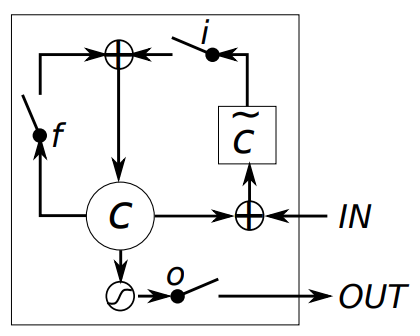
\includegraphics[width=5cm]{litReview/images/LSTM} }}%
  \qquad
  \subfloat[Gated Recurrent Unit]{{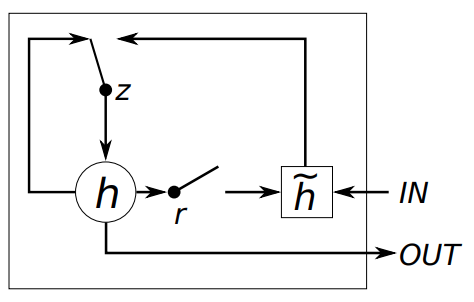
\includegraphics[width=5cm]{litReview/images/GRU} }}%
  \caption{Illustration of (a) LSTM and (b) gated recurrent units}%
  \label{fig:LSTM-GRU}%
  \citep{gru}
\end{figure}

\subsection{Convolutional Neural Network}

Although sequence-based models such as the RNN have proven significant results in text classification and other NLP related tasks, Convolutional Neural Networks (CNNs) can be advantageous due to their ability in extracting position invariant features \citep{CNNvsRNN}. CNNs have largely been applied to computer vision-related tasks, thus, it's important to note that techniques with regards to NLP and text classification differ to some extent \citep{DBLP:journals/corr/0001KYS17}.  
Furthermore, one of the major drawbacks of using sequence-based models is that they are blatantly slow to train. CNNs however, process elements simultaneously which in return speeds up the training process \citep{ghelani_2019}. Within CNNs, the convolution results will signal when a unique pattern is detected. These patterns could be expressions such as "I love" or "That sounds fantastic" etc in which CNNs can identify such phrases within a sentence regardless of its position. Due to this, CNNs are suitable for classification tasks such as sentiment analysis and spam detection \citep{ghelani_2019}. Concerning text classification, \citep{kim-2014-convolutional} showed that a simple CNN with little hyperparameter tuning achieved excellent results when applied to sentence classification. Additionally, \citep{1609.02748} demonstrated convincing results when employing a CNN for aspect extraction and sentiment analysis. It's important to note that the results obtained by \citep{kim-2014-convolutional} and \citep{1609.02748}  were not attained by CNNs alone, however, benefitted from the use of transfer learning along with word embedding techniques. 

\begin{figure}[H]
  \centering
  \includegraphics*[ width=1\linewidth]{litReview/images/cnn4text}
  \caption{Example of a CNN for text classification.}
  \label{fig:cnn4text}
  \citep{dennybritz}
\end{figure}

\section{Transfer Learning}

Collecting data is a complicated and expensive process which in return makes it difficult to build large-scale and high quality annotated datasets \citep{TransferLearning}. This problem of insufficient training data applies to various domains such as emotion classification from text as there is a lack of available annotated data \citep{emodetect-review}. When using a scarce dataset, it's evident that teaching a machine to learn the numerous grammatical nuances, cultural differences, sarcasm, and slang is an extremely difficult process. Transfer learning addresses this issue of insufficient training data by transferring knowledge from a different domain to the task at hand such that the pre-trained weights can be applied to the target domain \citep{TransferLearning}. For example, we can imagine that learning to classify apples may help us in learning to recognize pears as we are leveraging the already existing knowledge learned from classifying apples to a related task \citep{TL-Survey2}. Some of the key areas where transfer learning is being considered and applied are in self-driving cars and speech recognition \citep{sebastianruder2019}. For example, companies such as Google and Udacity are applying transfer learning by allowing their models to learn from virtual environments in which the acquired knowledge is then transferred to the real world \citep{sebastianruder2019}. With regards to text, however, transfer learning has mainly been applied in relation to language modeling and word embedding techniques \citep{pdf:nlpsurvery}.  

\begin{figure}[H]
  \centering
  \includegraphics*[ width=.6\linewidth]{litReview/images/transfer-learning}
  \caption{Learning process of transfer learning.}
  \label{fig:transfer-learning}
  \citep{TransferLearning}
\end{figure}

\subsection{Word Embeddings}

Simplistic models of transfer learning utilizing just a single layer of weights has been extremely popular for various years \citep{fastaiNLP}. Two of the most common techniques are Word2Vec and GloVe. Word2Vec, introduced by Google in 2013, is a word embedding model for computing continuous representations of words from extremely large datasets \citep{word2vec}. While Word2Vec can learn embeddings by relating target words to their context, it fails at recognizing whether some context words appear together more often than others \citep{word2vec-glove-fasttext}. Conversely, GloVe (Global Vectors for Word Representation), introduced by Stanford in 2014, creates a global co-occurrence matrix by estimating the probability that a given word will occur with other words \citep{glove}. Word embeddings are crucial to text classification as they turn text into a numerical format that deep neural networks are able to understand.

\noindent
\\ The above-mentioned word embedding techniques don't perform sufficiently on their own. Rather, these techniques have proven significant results when being able to inject knowledge from a larger corpus. For example, the already mentioned sentence level classifier using a CNN by \citep{kim-2014-convolutional} trained their one layer convolution using Word2Vec in which vectors were trained on 100 billion words of Google News. \cite{sarcastic-tweets} also make use of the publicly available Word2Vec vectors trained on Google News as a means to classify sarcasm in tweets using deep CNNs. 

\subsection{Language Modeling}

Though pre-trained word embeddings have been extremely influential, a major limitation is that they are trained on a neural network with one hidden layer, meaning that any previous knowledge can only be extracted from the first layer of the model \citep{nlp-imagenet}. As quoted by Jeremy Howard and Sebastian Ruder from FastAI, \textit{"only using transfer learning for a single layer is clearly just scratching the surface of what’s possible"} \citep{fastaiNLP}. Language modeling is an NLP model that tries to predict the next word in a sentence, hence, is advantageous in comparison to static word embedding approaches such as Word2Vec and GloVe as it forces the model to use information from the entire sentence. Like with word embeddings, language models are typically trained with extremely large datasets, however, in an unsupervised manner which in return allows them to capture the syntactic features more deeply than word embeddings \citep{language-modeling}. Most notably, \citep{DBLP:journals/corr/abs-1801-06146} proposed Universal Language Model Fine-tuning (ULMFiT) for text classification. The ULMFiT model enables you to train the language model on an extremely large dataset in order to capture features of the language in different layers, as well as to fine-tune the language model on the target domain using discriminative fine-tuning and slanted learning rates to learn domain-specific features. The stages of the model are further portrayed in Figure~\ref{fig:ulmfit}. ULMFiT was shown to significantly outperform the state-of-the-art on six text classification tasks and showed that by using only 100 labeled examples, it matched the performance of training from scratch on 100x more data \citep{DBLP:journals/corr/abs-1801-06146}. Only shortly after the release of ULMFiT, similar models with different architectures were released, nevertheless, with pre-trained language models being at the core of the structure. 

\begin{figure}[H]
  \centering
  \includegraphics*[ width=1\linewidth]{litReview/images/ULMFiT}
  \caption{ULMFiT stages.}
  \label{fig:ulmfit}
  \citep{DBLP:journals/corr/abs-1801-06146}
\end{figure}

\subsection{Attention Mechanisms \& The Transformer}

 As discussed in section 1.2, RNNs have proven impressive results in various sequence modeling tasks, however, they face limitations due to their inability in storing information about past features for a long time as well as the inability to provide higher weight to more important words. A solution to this problem was proposed by \citep{attention} where they introduced the model of \textit{self-attention}. The idea behind self-attention is to place "attention" towards words that are important to the meaning of the sentence. The representation of these instructive words is then formed into a sentence vector. Perhaps the most significant models where self-attention has been applied is in that of ELMo (Embeddings from Language Models) and transformer-based architectures such as BERT (Bidirectional Encoder Representations from Transformers) \citep{DBLP:journals/corr/abs-1810-04805}, Transformer-XL \citep{DBLP:journals/corr/abs-1901-02860} and Open AI's GTP-2 \citep{radford2019language}. 

 \noindent
\\ With regards to text classification, \citep{DBLP:journals/corr/abs-1906-09821} applied both ELMo and BERT as a means to classify and cluster
topic-dependent arguments and achieved compelling results. Their results indicate a captivating advantage in using contextualized word embeddings as opposed to previous word embedding approaches such as Word2Vec and GloVe.

 \subsubsection{ELMo}

 ELMo is designed such that is uses a deep bidirectional LSTM pre-trained on a large text corpus to learn context-dependent word representations \citep{Peters:2018}. Furthermore, ELMo representations are purely character-based allowing it to handle out of vocabulary words. ELMo showed to significantly improve the state-of-the-art for multiple NLP related tasks. 

 \begin{table}[h!]
  \begin{center}
    \begin{tabular}{ |c|c|c|c|c|c| }
    \hline
      \textbf{Task} & \textbf{Previous SOTA} & \textbf{ELMo} & \textbf{Increase} \\ 
    \hline
      SQuAD & SAN 84.4 & 85.8 & 1.4\% \\  
      SNLI & \citep{DBLP:journals/corr/ChenZLWJ16} 88.6 & 88.7+/-0.17 & 0.1\% \\ 
      SRL & \citep{he-etal-2017-deep} 81.7 &  84.6 & 2.9\% \\ 
      Coref & \citep{DBLP:journals/corr/LeeHLZ17} 67.2 &  70.4 & 3.2\% \\
      NER & \citep{DBLP:journals/corr/PetersABP17} 91.93+/0.19 &  92.22+/-0.10 & 0.29\% \\
      SST-5 & \citep{DBLP:journals/corr/abs-1708-00107} 53.7 & 54.7+/-0.5 & 1.0\% \\
    \hline 
    \end{tabular}
    \caption{ELMo results vs. previous state-of-the-art.}
    \label{table:1}
    \citep{Peters:2018}
  \end{center}
\end{table}

\subsubsection{BERT}

BERT built on top of ELMo by pre-training deep bidirectional representations from unlabeled text using the transformer architecture to compute word embeddings \citep{DBLP:journals/corr/abs-1810-04805}. Unlike ELMo, BERT uses masked language modeling and next sentence prediction for pre-training. BERT also proved to notably improve the state-of-the-art and showed better results in various tasks in comparison to ELMo.

\begin{table}[h!]
  \begin{center}
    \begin{tabular}{ |c|c|c|c|c|c| }
    \hline
      \textbf{Task} & \textbf{ELMo} & \textbf{BERT Large} & \textbf{BERT Base} & \textbf{Increase} \\ 
    \hline
      NER & 92.2 & 92.8 & 92.4 & 0.4\% \\
      SQuAD & 85.8 & 93.2 & 91.8 & 6.7\% \\
      SST-2 & 90.4 & 94.9 & 93.5 & 3.8\% \\
      CoLA & 36.0 & 60.5 & 52.1 & 20.3\% \\
      QNLI & 79.8 & 92.7 & 90.5 & 11.8\% \\
    \hline 
    \end{tabular}
    \caption{BERT vs ELMo on NLP tasks.}
    \label{table:1}
    \citep{DBLP:journals/corr/abs-1810-04805}
  \end{center}
\end{table}

\noindent
\\ While it may seem that these attention based models are superior to previous approaches, \citep{fastaiNLP} state that recurrent models such as ULMFiT still outperforms transformers on smaller datasets. 

\section{Datasets}

\subsection{Labeled Text}

As was discussed in section 1.3, emotion detection from text faces the issue of having a lack of publicly available annotated data. In terms of labeled text, one of the most common resources is ISEAR, International Survey On Emotion Antecedents And Reactions. The ISEAR dataset consists of 3000 responses from people around the world in which they were asked to recall experiences which triggered at least one of the seven emotions depicted from \citep{pdf:PaulEkmanEmotions} and \citep{plutchik1980general}, i.e. anger, anticipation, joy, trust, fear, surprise, sadness, and disgust. This resulted in a dataset containing a total of 7600 instances of text conveying emotional states. Another more common dataset that has been used is SemEval-2018 Task 1 E-c. This resource consists of 6,857 tweets with binary labels for eight of the Plutchik classes as well as 3 more (optimism, pessimism, and love) \citep{mohammad-etal-2018-semeval}. The SemEval-2007 Task 14 focused on affective text is another dataset which has been frequently used \citep{emodetect-review}. It contains a total of 1250 annotated news headlines drawn from well-known newspapers such as the New York Times, BBC News, CNN as well as Google News. Both the SemEval-2007 and 2018 tasks have mainly been used as benchmarks for comparing results achieved by different models. The lack of publicly available annotated data has largely pushed researchers and practitioners to mine text from social media sources such as Twitter where exposing emotion is possible through features such as hashtags and emoticons \citep{emodetect-review}. Due to the lack of publicly available annotated data, it's crucial to consider incorporating the previously mentioned transfer learning approaches with regards to word embeddings and language modeling as this may allow deep neural networks to better "understand" the training text which in return could improve the overall performance in emotion detection. 

\subsection{Pre-trained Word Embeddings}

Researchers behind the common word embedding models have open-sourced multiple pre-trained word embedding models for other researchers and practitioners to make use of. Table \ref{table:3} displays some of these pre-trained word embeddings. The first row shows the properties of a Word2Vec model trained on a Google News corpus consisting of 100B words with 300-dimensional vectors for approximately 3M words and phrases \citep{word2vec}. Additionally, we see that fastText distributes pre-trained vectors for both a Wikipedia and CommonCrawl corpus. The Wikipedia version consists of 16B tokens along with 300-dimensional vectors for 1M words, whilst the CommonCrawl version contains 600B tokens with 300-dimensional vectors for 2M words \citep{mikolov2018advances}. Furthermore, we can see that GloVe issues pre-trained vectors for a Twitter, and Wikipedia combined with Gigaword corpus as well as two separate adaptations for a CommonCrawl corpus. The Twitter model is trained on 27B tokens with 300-dimensional vectors for 1.2M words. The Wikipedia and Gigaword combination is trained on 6B tokens with 300-dimensional vectors on 400,000 words. Lastly, the CommonCrawl versions are trained on both 42B tokens with 300-dimensional vectors for 1.9M words as well as 840 billion tokens with 300-dimensional vectors for 2.2M words \citep{glove}. 

\begin{table}[h!]
\begin{center}
  \begin{tabular}{ |c|c|c|c|c|c| }
  \hline
    \textbf{Corpus} & \textbf{Type} & \textbf{Size} & \textbf{Vocab size} & \textbf{Dim} & \textbf{Download}  \\ 
  \hline
    Google News & Word2Vec & 100B & 3M & 300 & \href{https://code.google.com/archive/p/Word2Vec/}{link} \\  
    Wikipedia & fastText & 16B & 1M & 300 & \href{https://fasttext.cc/docs/en/english-vectors.html}{link} \\ 
    CommonCrawl & fastText & 600B & 2M & 300 & \href{https://fasttext.cc/docs/en/english-vectors.html}{link} \\ 
    Twitter & GloVe & 27B & 1.2M & 300 & \href{https://nlp.stanford.edu/projects/glove/}{link} \\
    Wikpedia + Gigaword & GloVe & 6B & 400K & 300 & \href{https://nlp.stanford.edu/projects/glove/}{link} \\
    CommonCrawl & GloVe & 42B & 1.9M & 300 & \href{https://nlp.stanford.edu/projects/glove/}{link} \\
    CommonCrawl & GloVe & 840B & 2.2M & 300 & \href{https://nlp.stanford.edu/projects/glove/}{link} \\
  \hline 
  \end{tabular}
  \caption{Word embedding model properties.}
  \label{table:3}
\end{center}
\end{table}

\subsection{Pre-trained Language Models}

Like with pre-trained word embeddings, various organizations have open-sourced their pre-trained language models. Below we specifically view the properties of the pre-trained ELMo models released by \citep{Peters:2018} and pre-trained BERT models released by \citep{DBLP:journals/corr/abs-1810-04805}. While there are other pre-trained language models to consider such as ones available with Transformer-XL \citep{DBLP:journals/corr/abs-1901-02860} and Open-AI's GTP-2 \citep{radford2019language}, ELMo and BERT seem to be more applicable to text classification. 

\subsubsection{Pre-trained ELMo Models}

Table \ref{table:4} displays all pre-trained ELMo models. 
All models except for the Original 5.5B model were trained on the \href{http://www.statmt.org/lm-benchmark/}{1 Billion Word Language Model Benchmark} which consists of approximately 800 million tokens of WMT 2011 News Crawl data. The ELMo 5.5B model was trained on a dataset containing 5.5B tokens of Wikipedia (1.9B) and all of the monolingual news crawl data from WMT 2008-2012 (3.6B) \citep{Peters:2018}.

\begin{table}[h!]
  \begin{center}
    \begin{tabular}{ |c|c|c|c|c|c| }
    \hline
      \textbf{Model} & \textbf{Parameters} & \textbf{Weights} \\ 
      \hline
      Small & 13.6M & \href{https://s3-us-west-2.amazonaws.com/allennlp/models/elmo/2x1024_128_2048cnn_1xhighway/elmo_2x1024_128_2048cnn_1xhighway_weights.hdf5}{weights} \\     
      Medium & 28.0M & \href{https://s3-us-west-2.amazonaws.com/allennlp/models/elmo/2x2048_256_2048cnn_1xhighway/elmo_2x2048_256_2048cnn_1xhighway_weights.hdf5}{weights} \\  
      Original & 93.6 & \href{https://s3-us-west-2.amazonaws.com/allennlp/models/elmo/2x4096_512_2048cnn_2xhighway/elmo_2x4096_512_2048cnn_2xhighway_weights.hdf5}{weights} \\  
      Original (5.5B) & 93.6 & \href{https://s3-us-west-2.amazonaws.com/allennlp/models/elmo/2x4096_512_2048cnn_2xhighway_5.5B/elmo_2x4096_512_2048cnn_2xhighway_5.5B_weights.hdf5}{weights} \\   
    \hline 
    \end{tabular}
    \caption{Pre-trained ELMo models.}
    \label{table:4}
    \citep{Peters:2018}
  \end{center}
\end{table}

\noindent
Further information about ELMo along with downloads for the pre-trained weights can be found at \url{https://allennlp.org/elmo}.

\subsubsection{Pre-trained BERT Models}

Table \ref{table:5} displays all pre-trained English BERT models.
Both the BERT-Base and BERT-Large models were trained on Wikipedia data with 2.5B words from text passages of English Wikipedia as well as \href{https://yknzhu.wixsite.com/mbweb}{BookCorpus} which is a dataset consisting of 11,038 unpublished books from 16 different genres \citep{DBLP:journals/corr/abs-1810-04805} \citep{moviebook}.  

\newpage
\begin{table}[h!]
  \begin{center}
    \begin{tabular}{ |c|c|c|c|c|c| }
    \hline
      \textbf{Model} & \textbf{Parameters} & \textbf{Weights} \\ 
      \hline
      Large, Uncased (Whole Word Masking) & 340M & \href{https://storage.googleapis.com/bert_models/2019_05_30/wwm_uncased_L-24_H-1024_A-16.zip}{weights} \\     
      Large, Cased (Whole Word Masking) & 340M & \href{https://storage.googleapis.com/bert_models/2019_05_30/wwm_cased_L-24_H-1024_A-16.zip}{weights} \\  
      Base, Uncased & 110M & \href{https://storage.googleapis.com/bert_models/2018_10_18/uncased_L-12_H-768_A-12.zip}{weights} \\  
      Large, Uncased & 340M & \href{https://storage.googleapis.com/bert_models/2018_10_18/uncased_L-24_H-1024_A-16.zip}{weights} \\   
      Base, Cased  & 110M & \href{https://storage.googleapis.com/bert_models/2018_10_18/cased_L-12_H-768_A-12.zip}{weights} \\
      Large, Cased & 340M & \href{https://storage.googleapis.com/bert_models/2018_10_18/cased_L-24_H-1024_A-16.zip}{weights} \\
    \hline 
    \end{tabular}
    \caption{Pre-trained BERT models.}
    \label{table:5}
    \citep{DBLP:journals/corr/abs-1810-04805}
  \end{center}
\end{table}

\noindent
Further information about BERT along with downloads for the pre-trained weights can be found at \url{https://github.com/google-research/bert}.

\section{Related Work}

A machine learning approach in the domain of emotion classification from text was done by \citep{EmoTxt}. They present a toolkit for emotion recognition from text where they specifically introduce an emotion lexicon designed to capture the presence of lexical cues that convey emotion in text. Using uni- and bi-grams with tf-idf weighting, they compute the tf-idf for each emotion category based on how many times they occur in WordNet affect, a lexical resource representing affective concepts in correlation with affective words. They train their classification models using Support Vector Machines (SVM) on a dataset containing 4,800 posts from Stack Overflow as well as 4000 commented posts by software developers on Jira. While having obtained sufficient results, they did not experiment with any deep learning approaches. 

\noindent
\\ A deep learning approach was introduced by \citep{senarath-thayasivam-2018-datasearch}. They describe a method to solve distinct emotion classification with the use of pre-trained word embedding models to train multiple neural networks along with an LSTM and CNN for feature extraction and feedforward neural network for classification. They specifically make use of Word2Vec, fastText and GloVe as their word-embedding algorithms. Their Word2Vec model was trained on both a Twitter corpus of 400 million tweets as well as the  Google News corpus of 100 billion words. Interestingly, they found that their model performed best when using Word2Vec trained on Twitter data making the hypothesis that the model performed better due to the pre-trained Twitter corpus consisting of similar vocabulary to their domain. A limitation of their approach is that their research did not focus on fine-tuning the model architectures to different word-embeddings. 

\noindent
\\ Furthermore, \citep{dl-affective} proposed "sent2affect", another transfer learning approach in which they utilize a source domain that is semantically similar to the target domain. The related task they decided to use was sentiment analysis as it shares some similarities in the sense that classifying text as either "positive" or "negative" is achieved from lexical content. Their approach differs from \citep{senarath-thayasivam-2018-datasearch} as they decided to feed the pre-trained word-embeddings solely into a RNN as opposed to a combination of an LSTM and CNN. They compare their sent2affect approach to a pre-trained embeddings approach with a bidirectional LSTM layer and show that sent2affect produced some additional performance improvements. 

\noindent
\\ The authors \citep{zhong2019ntuer} presented a model to detect emotion from textual conversations. They compare the results obtained from using a Recurrent Convolutional Neural Network (RCNN) along with pre-trained word embeddings to those attained from using ELMo and BERT as their pre-trained language models. Interestingly, they found that the pre-trained language models performed worse in comparison to the RCNN. Their model was applied to classify emotions into just four different categories (happy, sad, angry and others), thus, results would likely be different if they were to attempt classifying into more labels. 

\noindent
\\ Lastly, the research done by \citep{1812.01207} demonstrated that multi-emotion sentiment can be classified using large pre-trained language models. Specifically, they train an attention-based transformer network on 50GB of Amazon reviews. In addition, they compare results obtained using an attention-based transformer to that achieved by a multiplicative LSTM (mLSTM) and show that the transformer generally out-performs the mLSTM. 

\section{Conclusions}

Upon reviewing the multiple variations of deep learning models and recent trends in NLP, it would seem that there are various paths one can take to tackle the task of emotion detection from text. The review showed that both sequence-based models and convolutional neural networks have demonstrated sufficient results in the domain of text classification and noted that while RNN variants such as the GRU and LSTM are able to retain crucial information for much longer, CNNs can be superior due to being able to extract position invariant features. Due to this, it would be suitable to compare and contrast results obtained from both models. Furthermore, the findings in the research on transfer learning showed that the collection of data with regards to emotion classification from text is a complicated and expensive process, however, this problem is relaxed when leveraging existing knowledge learned from a different domain to the task at hand. Specifically, the review showed that the use of pre-trained word embedding and pre-trained language models have proved to significantly improve the state-of-the-art in multiple NLP related tasks. In addition, multiple researchers and organizations have open sourced their variations for pre-trained word embedding and pre-trained language models which can be fine-tuned on small NLP tasks such as emotion detection. Therefore, these techniques would present a feasible approach for the area of research. 




\chapter{Experiment Design}\label{ch:Requirements Analysis}

This chapter details the experimental setup for carrying out the task of classifying emotion from text. In particular, the chapter outlines the text pre-processing steps, the model architecture, evaluation metrics and technologies that are made use of.

\section{Data}

This study makes use of both the \textit{ISEAR} (International Survey on Emotion Antecedents And Reactions) and \textit{SemEval-2018 Affect In Tweets} datasets. The ISEAR dataset consists of 3000 responses from people around the world who report situations where they experienced each of the emotions from (joy, fear, anger, sadness, disgust, shame, and guilt). The dataset is split such that 80\% is assigned to the training set, 10\% to the validation set and the last 10\% to the testing set. 

\subsection{Pre-trained Word Embeddings \& Language Models}

Due to the minimal amount of training data, we make use of the pre-trained GloVe embeddings trained on the Wikipedia and Gigaword corpus \textit{(6B tokens, 400k vocab, uncased, 300d)}, the pre-trained Word2Vec embeddings trained on the Google News corpus \textit{(100B words, 3M vocab, 300d)} as well as the ELMo embeddings trained on the 1 Billion word benchmark available from \href{https://tfhub.dev/}{Tensorflow-Hub}. Furthermore, the \href{https://github.com/huggingface/transformers}{Huggingface Transformers} library for Tensorflow is utilized in order to retrieve the pre-trained BERT model and to compute BERT embeddings. 

\subsection{Pre-processing}

Text in which people recall experiences likely consists of various informal words and words which don't have any significant correlation towards the emotions being conveyed. Thus, keeping these words in the text increases the overall feature dimensionality. As a means to counter this issue, this study makes use of text pre-processing techniques such as stop-word removal, removing punctuations and accent marks, removing white spaces, and likewise to \citep{DBLP:journals/corr/abs-1801-06146}, adding special tokens for upper-case words and repetition as this may allow the model to capture characteristics which are important to classification.

\section{Models}

As shown by the enumerated list below, the overall model architecture is designed such that it contains the following layers: 

\begin{enumerate}
  \item Pre-trained embeddings layer 
  \item Model layer 
  \item Dropout layer 
  \item Classification layer 
\end{enumerate}

\noindent
The embedding layer is initialized using pre-trained Word2Vec, ELMo and BERT embeddings such that the pre-processed input text from the dataset is converted into an embedding representation. Furthermore, the model layer makes use of an RNN, CNN and RCNN. With regards to the RNN, the experiment is carried out using both a unidirectional LSTM as well as a bidirectional LSTM. The RCNN architecture proposed by \citep{AAAI159745} is used in order to take advantage of both the RNN and CNN as a means to further improve the emotion classification. Next, the dropout layer is implemented in order to ensure that the model does not over-fit the data. Lastly, the classification layer makes use of Cross-Entropy loss in order to compute the probabilities of the input text belonging to each of the class labels. 

\begin{figure}[H]
  \centering
  \includegraphics*[ width=1\linewidth]{methodology/images/design.png}
  \caption{Proposed architecture.}
  \label{fig:bert-model}
\end{figure}

\noindent
Furthermore, we compare the result of the above mentioned Deep Learning models to that of machine learning algorithms such as Logistic Regression. We apply the machine learning algorithms using Term Frequency Inverse Document Frequency (TF-IDF) as a means to convert text into vector form. 

\section{Performance Evaluation}

This study evaluates the performance of all models using accuracy and the micro and macro F1 scores. We specifically optimize each model with the micro and macro F1 scores in mind. This is because the dataset consists of labels with more instances than others. Furthermore, the micro and macro F1 scores have been used in various other papers that tackle the task of emotion classification from text \citep{paperswithcode}. Therefore, these metrics provide a good comparison for the overall performance of the models implemented in this study. 

\begin{equation}
  PREmicro = \frac{TP1 + TP2}{TP1 + TP2 + FP1 + FP2}
\end{equation}

\begin{equation}
  RECmicro = \frac{TP1 + TP2}{TP1 + TP2 + FN1 + FN2}
\end{equation}

\noindent
\\ The micro F1 score is equal to the harmonic mean of these two figures \citep{shams_1970}.

\begin{equation}
  PREmacro = \frac{PRE1 + PRE2}{2}
\end{equation}

\begin{equation}
  RECmacro = \frac{REC1 + REC2}{2}
\end{equation}

\noindent
\\ The macro F1 score is equal to the harmonic mean of these two figures \citep{shams_1970}. 

\section{Technologies}

The experiment makes use of Python along with Tensorflow and Keras for constructing the architecture of the models. Both the Natural Language Toolkit (NLTK), and Keras Tokenizer libraries are used for text pre-processing. The Scikit learn library is used for the implementation of machine learning models. 





  
% \chapter{Design}\label{ch:Design}

This chapter examines the design of the project.

\section{Conclusions}

The main conclusions for this chapter.



% \chapter{Implementation}\label{ch:Implementation}

This chapter examines the implementation of the project.

\section{Conclusions}

The main conclusions for this chapter.



% \chapter{Evaluation \& Testing}\label{ch:Evaluation}

This chapter evaluates the overall project and provides results of tests carried out.

\section{Conclusions}

The main conclusions for this chapter.



% \chapter{Conclusion}\label{ch:Conclusion}

This chapter summarises the main outcomes and conclusions resulting from this body of work.

\section{Conclusions}

The main conclusions that may be drawn from the body of work.

\section{Future Work}

Further development that could be carried out in the future.


\footnotesize
\bibliographystyle{agsm}
\bibliography{thesis}
\normalsize
\appendix
% \chapter{Project Specification}
Summary of the project outline.

\section{Functional Requirements}
some text here

\section{Non-Functional Requirements}
some text here

\chapter{Project Management}
Discussion on how the project was managed. What things impacted the success of the project. How does the continually revised versions of the project plan compare to the initial draft developed at the start of the project. Did everything run according the schedule. Did elements such as exams \& coursework have any impact. 

\chapter{Another Appendix}

This appendix makes use of the \emph{rotating} package to rotate both figures and tables ninety degrees allowing for large datasets and illustrations to be represented.

\begin{sidewaystable}
\begin{center}
   \begin{tabular}{llllllllll} 
   \toprule
   \textbf{Heading 1} & \textbf{Heading 2}  & \textbf{Heading 3}  & \textbf{Heading 4}  & \textbf{Heading 5}  & \textbf{Heading 6}  & \textbf{Heading 7}  & \textbf{Heading 8}  & \textbf{Heading 9}  & \textbf{Heading 10}  \cr
   \midrule
   aaa & bbbb & cccc & dddd & eeee & ffff & gggg & hhhh & iiii & jjjj \cr 
   aaa & bbbb & cccc & dddd & eeee & ffff & gggg & hhhh & iiii & jjjj \cr 
   aaa & bbbb & cccc & dddd & eeee & ffff & gggg & hhhh & iiii & jjjj \cr 
   aaa & bbbb & cccc & dddd & eeee & ffff & gggg & hhhh & iiii & jjjj \cr 
   aaa & bbbb & cccc & dddd & eeee & ffff & gggg & hhhh & iiii & jjjj \cr 
   aaa & bbbb & cccc & dddd & eeee & ffff & gggg & hhhh & iiii & jjjj \cr 
   \bottomrule
   \end{tabular}
\caption[A Short Caption for the table]{
	A much longer caption that will not be listed in the list of tables page.
}
\label{tab:sidewaysTable}
\end{center}
\end{sidewaystable}

\begin{sidewaysfigure}
\centerline{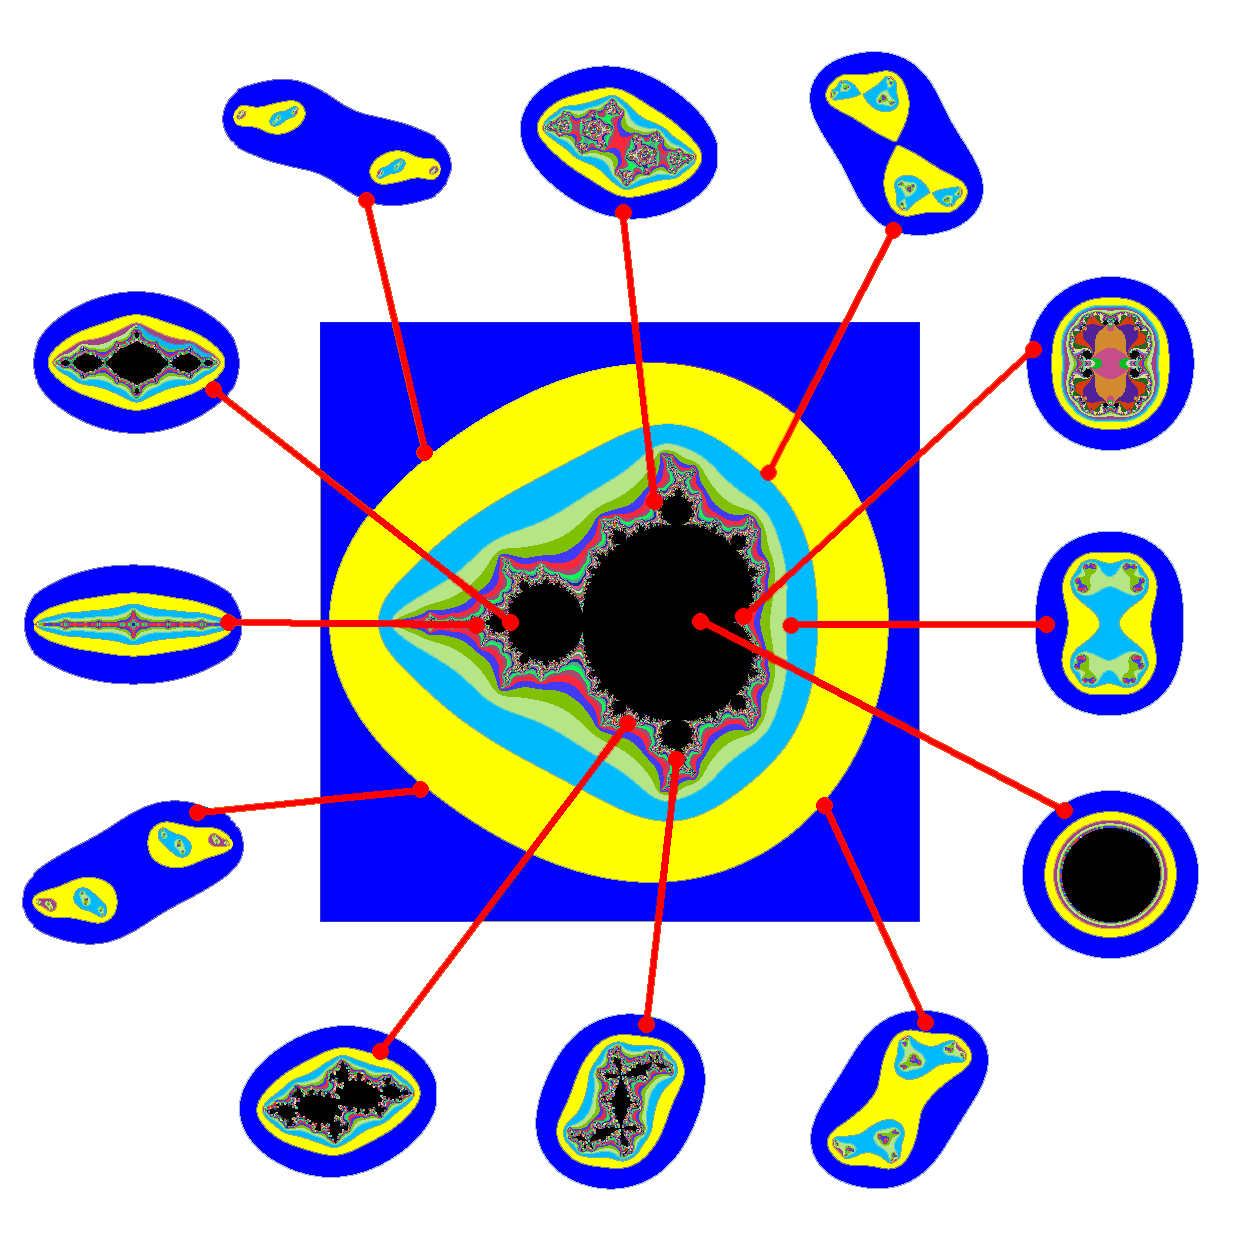
\includegraphics[width=7in]{appendix/images/samplepng}}
\caption[A Sideways Figure]{
	A much longer caption that will not be listed in the list of figures page.
}
\label{fig:sidewaysFigure}
\end{sidewaysfigure}

\chapter{Presentation Slides}

The slides from the formal presentation should be provided here in not more than two pages. 

\chapter{Project Log}

The following is a weekly summary of the work carried during the development of this body of work. It covers tasks that were completed, tutorials that were worked through, articles that were read and reviews of discussions / meetings held with the project supervisor and other third parties. 

\section*{Week Beginning: Monday 27/09/2010}

First week working on the project. Had a meeting with supervisor and discussed some of the issues related to the project. The first deliverable is due for the end of next week (project outline \& ethics form). 

\begin{itemize}
  \item Downloaded and Installed \LaTeX \space (MikTeX full install), Ghostscript, Ghostview \& Winshell. 
  \item Started to get to grips with the \LaTeX \space system by making simple modifications to the template and editing the project log.
  \item Developed a Mind Map to clarify understanding of project elements.
  \item Prepared an initial draft of project plan in the form of a Gantt chart. 
  \item Prepared and revised 1 page draft of project summary \& filled in ethics form. 
\end{itemize}




\end{document}